\chapter{Discussion}
\section{Water Year 2019} 
\subsection{Isothermal Snowpack and Peak Runoff Timing}
When a snowpack goes isothermal at 0C, all the energy input goes directly to snowmelt. Because of this, an isothermal snowpack is often critical in predicting major runoff timing. According to the Banner Summit Temperature Array, the snowpack reaches isothermal conditions on April 3, 2019 and this directly corelates with major runoff show in Figure \ref{fig:ValleyCreek} shows unregulated streamflow at a USGS stream gage near Banner Summit. 

\begin{figure}
    \centering
    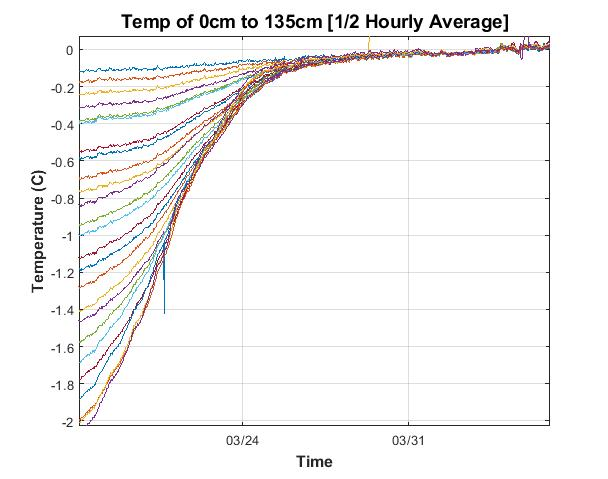
\includegraphics[width=0.7\linewidth]{figures/0_135cm_Isothermal.jpg}
    \caption{Progression of snowpack temperatures leading to isothermal conditions.}
    \label{fig:0_135cm_Isothermal}
 \end{figure}
 
 \begin{figure}
    \centering
    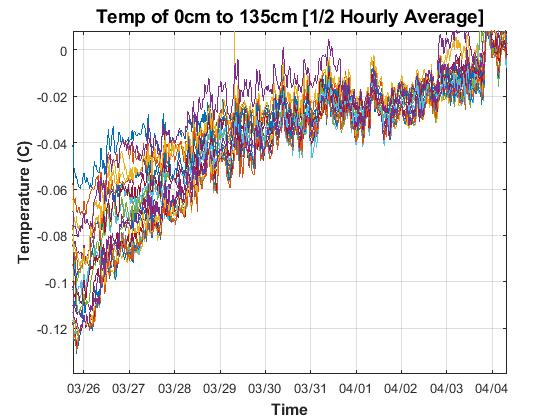
\includegraphics[width=0.7\linewidth]{figures/0_135cm_zoom.jpg}
    \caption{Sub-plot of data shown in Figure \ref{fig:0_135cm_Isothermal}}
    \label{fig:0_135cm_Zoom}
 \end{figure}

\begin{figure}
    \centering
    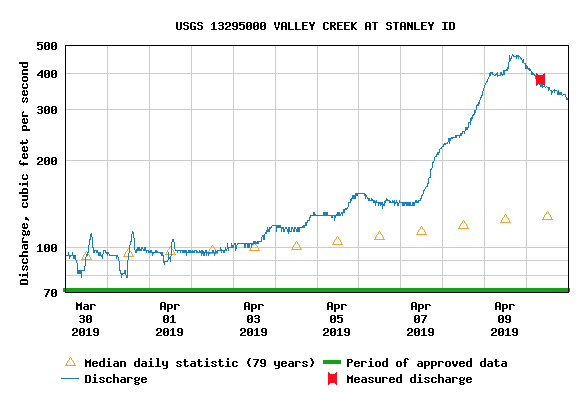
\includegraphics[width=0.8\linewidth]{figures/ValleyCreek_Gage.png}
    \caption{\textbf{Valley Creek} Unregulated streamflow data from a USGS gage near Banner Summit.}
    \label{fig:ValleyCreek}
 \end{figure}

\subsection{Stable Water Isotopes}
The 2019 isotope data have some significant random error because samples were taken in a lightly forested area with varying amounts of underbrush and fallen trees. This uneven ground creates an inconsistent datum between sampling events and introduces an unexpected amount of spatial variability. In addition to this, stable water isotopes could be effected by nearby trees and buried brush that emit longwave radiation. Moving forward, sampling for stable water isotopes in snow should be conducted open areas with an even ground surface that is free of large brush, or fallen debris. If a study is conducted in a forested/lightly forested area, there should be a preseason effort to clear the sampling locations of anything that makes the sampling locations uneven. 

- Interpretability of WY2019 isotope dataset \\
- Future directions  \\
- Coupling temperature and isotope dataset \\
